\documentclass{article}
\usepackage[T1]{fontenc}
\usepackage{lmodern}
\usepackage{graphicx}
\usepackage{amsmath,amssymb}
\usepackage[a4paper,margin=2cm]{geometry}
\usepackage[absolute,overlay]{textpos}
\setlength{\TPHorizModule}{1mm}
\setlength{\TPVertModule}{1mm}
\usepackage[indonesian]{babel}
\usepackage{hyperref}
\setlength{\emergencystretch}{2em}
\title{20-Steganografi-Bagian2-2026}
\author{pdf\_ppt\_to\_latex}
\date{}

\begin{document}

% --- unit llm 1 ---
% === Halaman 1 (llm) ===

\begin{center}
IF4020 Kriptografi

\Huge \textcolor{red}{20 - Steganalisis}

\vspace{40mm}

\large Oleh: Rinaldi M

\vspace{10mm}

Program Studi Teknik Informatika \\
Sekolah Teknik Elektro dan Informatika \\
Institut Teknologi Bandung \\
2026
\end{center}

\newpage

% --- unit llm 2 ---
% === Halaman 2 (llm) ===

\section*{Steganalysis}

\vspace{101.57mm}

\begin{itemize}
    \item Tujuan: menentukan apakah sebuah media \textit{suspect} mengandung pesan tersembunyi
\end{itemize}

\vspace{10mm}

% deskripsi: Ilustrasi proses steganalysis yang menunjukkan penggunaan kaca pembesar untuk melihat nilai-nilai piksel (angka digital) di dalam sebuah gambar wajah seseorang.
% bbox normalisasi: [0.2910, 0.4560, 0.5930, 0.7980]
\begin{textblock*}{63.42mm}(61.11mm,135.43mm)
\noindent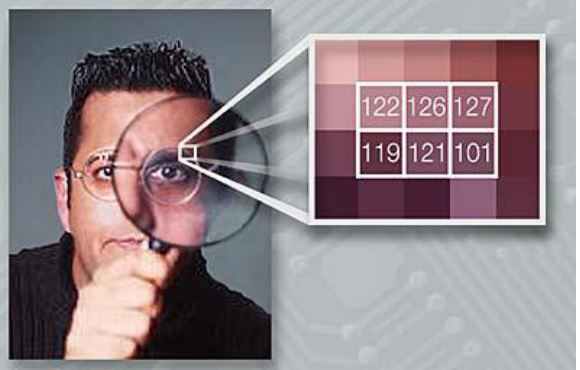
\includegraphics[width=63.42mm,height=101.57mm]{images/llm/page_002_img_01.png}%
\end{textblock*}

\newpage

% --- unit llm 3 ---
% === Halaman 3 (llm) ===

\vspace{83.46mm}

\begin{itemize}
    \item Steganografi
\end{itemize}
\vspace{60mm}
\begin{itemize}
    \item Steganalisis
\end{itemize}
\vspace{30mm}
*) Keterangan: 1 jika ada pesan tersembunyi, 0 jika tidak

\vspace{23.76mm}

% deskripsi: Diagram proses steganografi yang menunjukkan aliran dari message dan cover-object melalui proses Embedding menggunakan key untuk menghasilkan stego-object, yang kemudian diproses oleh adversary atau di-extract menggunakan key untuk mendapatkan kembali message.
% bbox normalisasi: [0.2170, 0.2020, 0.7510, 0.4830]
\begin{textblock*}{112.14mm}(45.57mm,59.99mm)
\noindent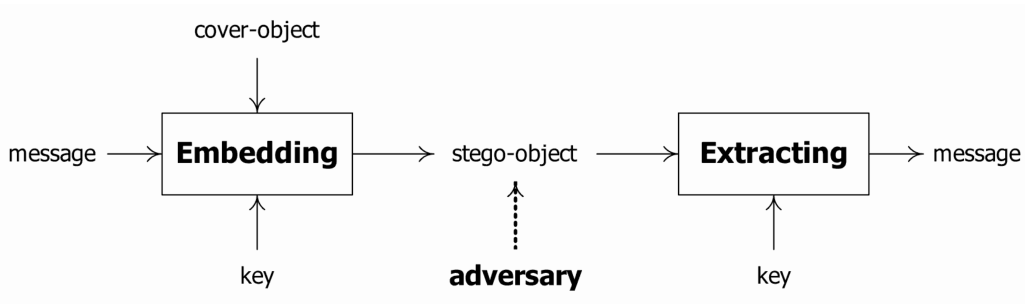
\includegraphics[width=112.14mm,height=83.46mm]{images/llm/page_003_img_01.png}%
\end{textblock*}

% deskripsi: Diagram proses steganalisis yang menunjukkan input berupa suspected stego object yang masuk ke blok Analisis untuk menghasilkan decision (1/0).
% bbox normalisasi: [0.2360, 0.6670, 0.6280, 0.7470]
\begin{textblock*}{82.32mm}(49.56mm,198.10mm)
\noindent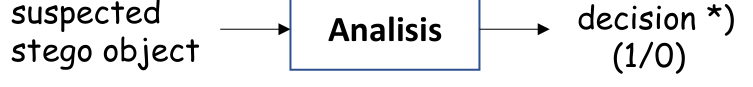
\includegraphics[width=82.32mm,height=23.76mm]{images/llm/page_003_img_02.png}%
\end{textblock*}

\newpage

% --- unit llm 4 ---
% === Halaman 4 (llm) ===

Fakta: Gambar-gambar bertebaran di internet
(website, social media, social networking)

\vspace{10mm}

% deskripsi: Screenshot postingan Facebook oleh Yogi Wahyu Prasida tentang kecelakaan kecil taksi otonom di Singapura.
% bbox normalisasi: [0.1520, 0.2780, 0.4780, 0.9250]
\begin{textblock*}{68.46mm}(31.92mm,82.57mm)
\noindent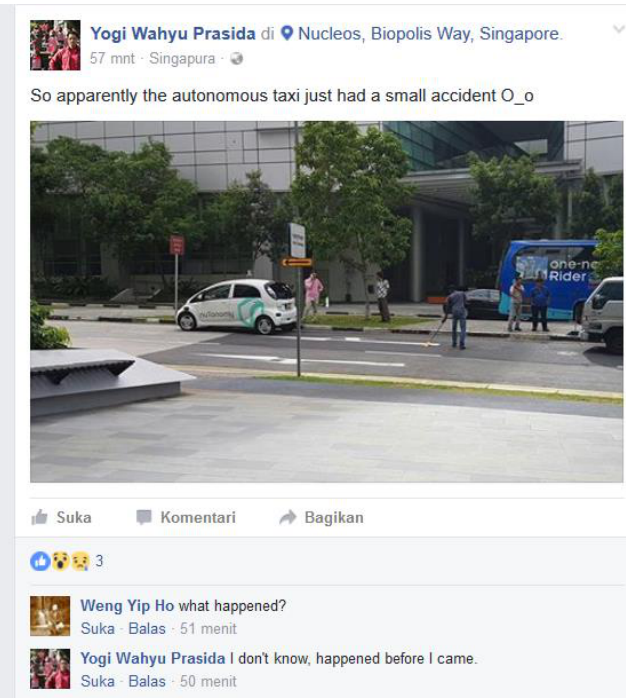
\includegraphics[width=68.46mm,height=192.16mm]{images/llm/page_004_img_01.png}%
\end{textblock*}

% deskripsi: Screenshot postingan Instagram oleh ashleyyukki yang menampilkan foto Jembatan Golden Gate.
% bbox normalisasi: [0.5780, 0.2780, 0.7840, 0.9320]
\begin{textblock*}{43.26mm}(121.38mm,82.57mm)
\noindent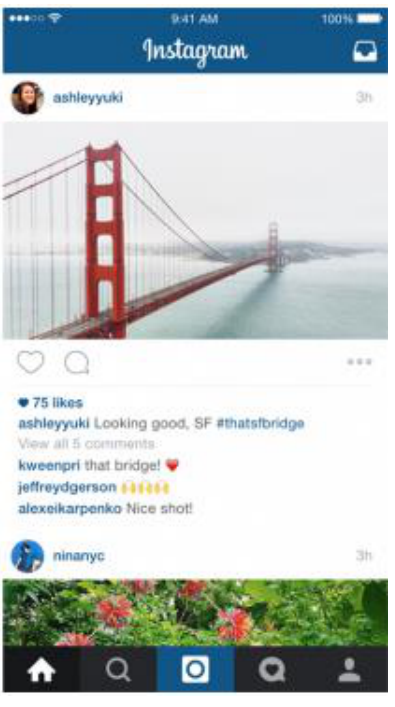
\includegraphics[width=43.26mm,height=194.24mm]{images/llm/page_004_img_02.png}%
\end{textblock*}

\newpage

% --- unit llm 5 ---
% === Halaman 5 (llm) ===

\vspace{149.39mm}

Namun, dibalik sebuah gambar dapat tersembunyi informasi rahasia
\vspace{60mm}
Informasi rahasia tersebut dapat berupa pesan biasa, pesan kejahatan, program jahat, bahkan virus komputer!

% deskripsi: Ilustrasi steganografi yang menunjukkan gambar Mona Lisa dengan panah yang mengarah ke sekumpulan kode biner dan teks 'VIRUS', melambangkan penyembunyian data rahasia di dalam gambar.
% bbox normalisasi: [0.2480, 0.2300, 0.6830, 0.7330]
\begin{textblock*}{91.35mm}(52.08mm,68.31mm)
\noindent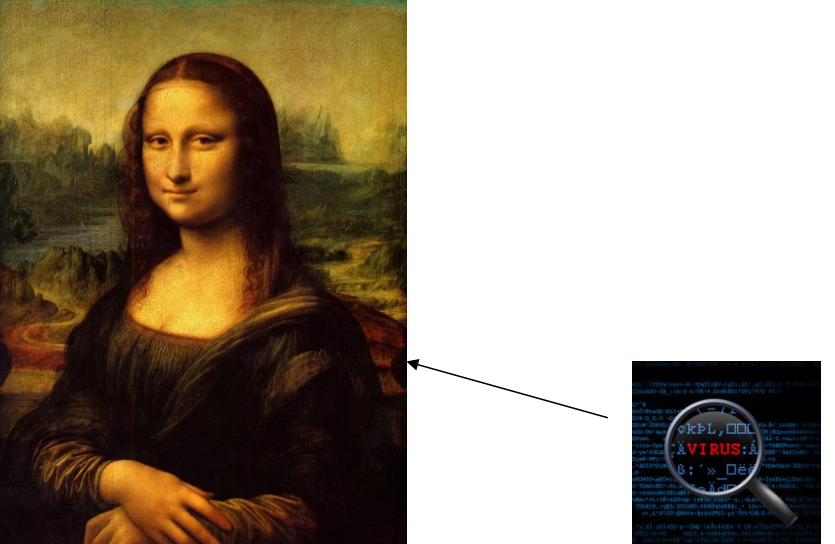
\includegraphics[width=91.35mm,height=149.39mm]{images/llm/page_005_img_01.png}%
\end{textblock*}

\newpage

% --- unit llm 6 ---
% === Halaman 6 (llm) ===

Pernah terima surel (\textit{e-mail}) dari orang tak dikenal dan mengandung \textit{file attachment} berupa gambar seperti di bawah ini?

\vspace{10mm}

\textbf{\color{red}HATI-HATI!!!!!!!!!!!}

% deskripsi: Screenshot contoh email phishing yang berisi lampiran gambar ucapan Tahun Baru 2016 dari 'Institute of Research Engineers and Doctors'.
% bbox normalisasi: [0.1780, 0.2760, 0.6540, 0.8730]
\begin{textblock*}{99.96mm}(37.38mm,81.97mm)
\noindent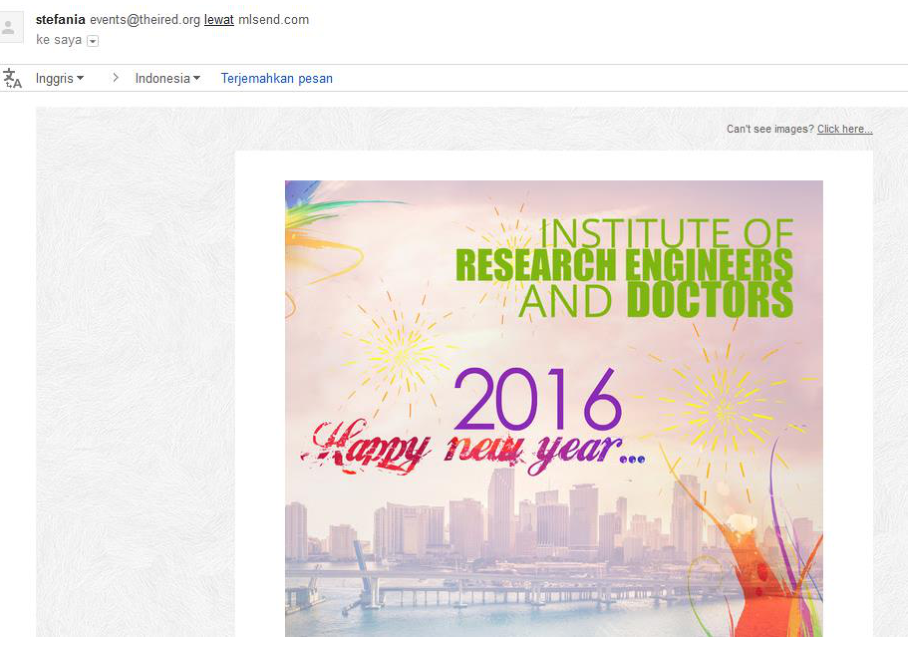
\includegraphics[width=99.96mm,height=177.31mm]{images/llm/page_006_img_01.png}%
\end{textblock*}

\newpage

% --- unit llm 7 ---
% === Halaman 7 (llm) ===

Hi rinaldi-m,

\vspace{20mm}

This message is sent on behalf of Benyamin Boy.
\small{Block future emails like this | Privacy policy}
\small{Zorpia Co. Ltd. P.O. Box \#28960, Gloucester Road Post Office, Hong Kong}

\vspace{10mm}

\centering{\textcolor{red}{\textbf{HATI-HATI! Jangan langsung klik jika anda tidak yakin!}}}

% deskripsi: Screenshot email phishing yang menunjukkan pesan palsu dari Benyamin dengan tombol 'Read Message' yang mencurigakan.
% bbox normalisasi: [0.1680, 0.1160, 0.8310, 0.6650]
\begin{textblock*}{139.23mm}(35.28mm,34.45mm)
\noindent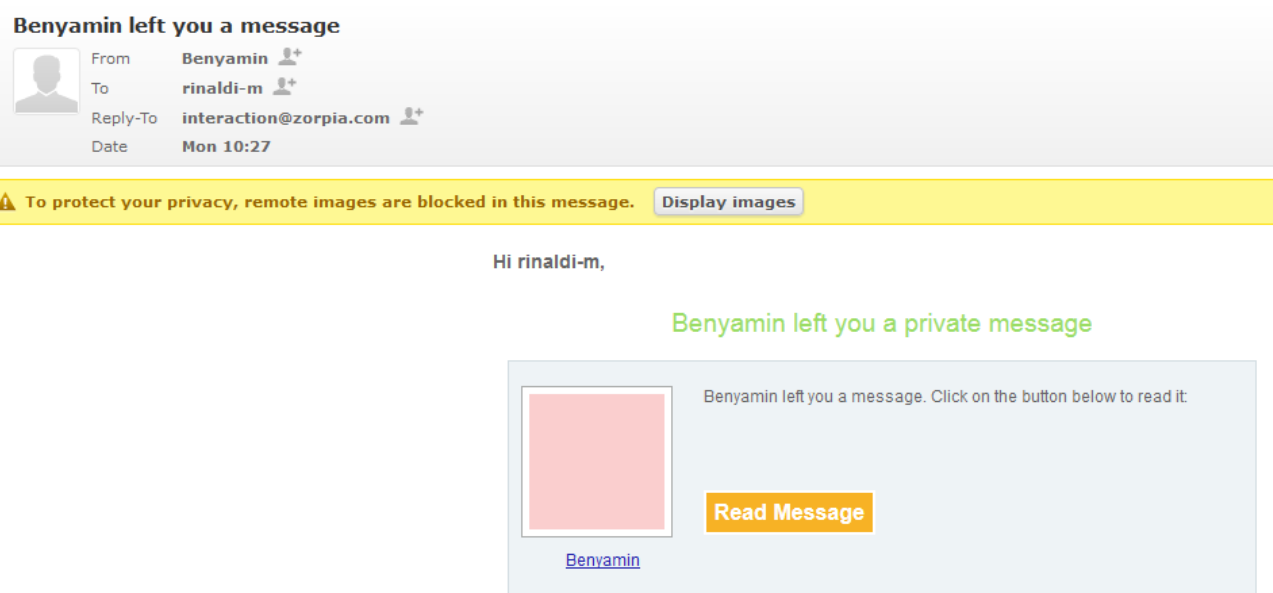
\includegraphics[width=139.23mm,height=163.05mm]{images/llm/page_007_img_01.png}%
\end{textblock*}

\newpage

% --- unit llm 8 ---
% === Halaman 8 (llm) ===

\vspace{238.79mm}

Ingat kembali stegosploit!!!

\vspace{10mm}

Just look at the image and you are HACKED!

\url{http://thehackernews.com/2015/06/Stegosploit-malware.html}

% deskripsi: Screenshot artikel berita tentang Stegosploit yang menunjukkan gambar kucing dengan teks overlay 'THIS PICTURE CAN HACK YOUR COMPUTER' dan penjelasan mengenai teknik menyembunyikan kode berbahaya dalam piksel gambar.
% bbox normalisasi: [0.0600, 0.1080, 0.9400, 0.9120]
\begin{textblock*}{184.80mm}(12.60mm,32.08mm)
\noindent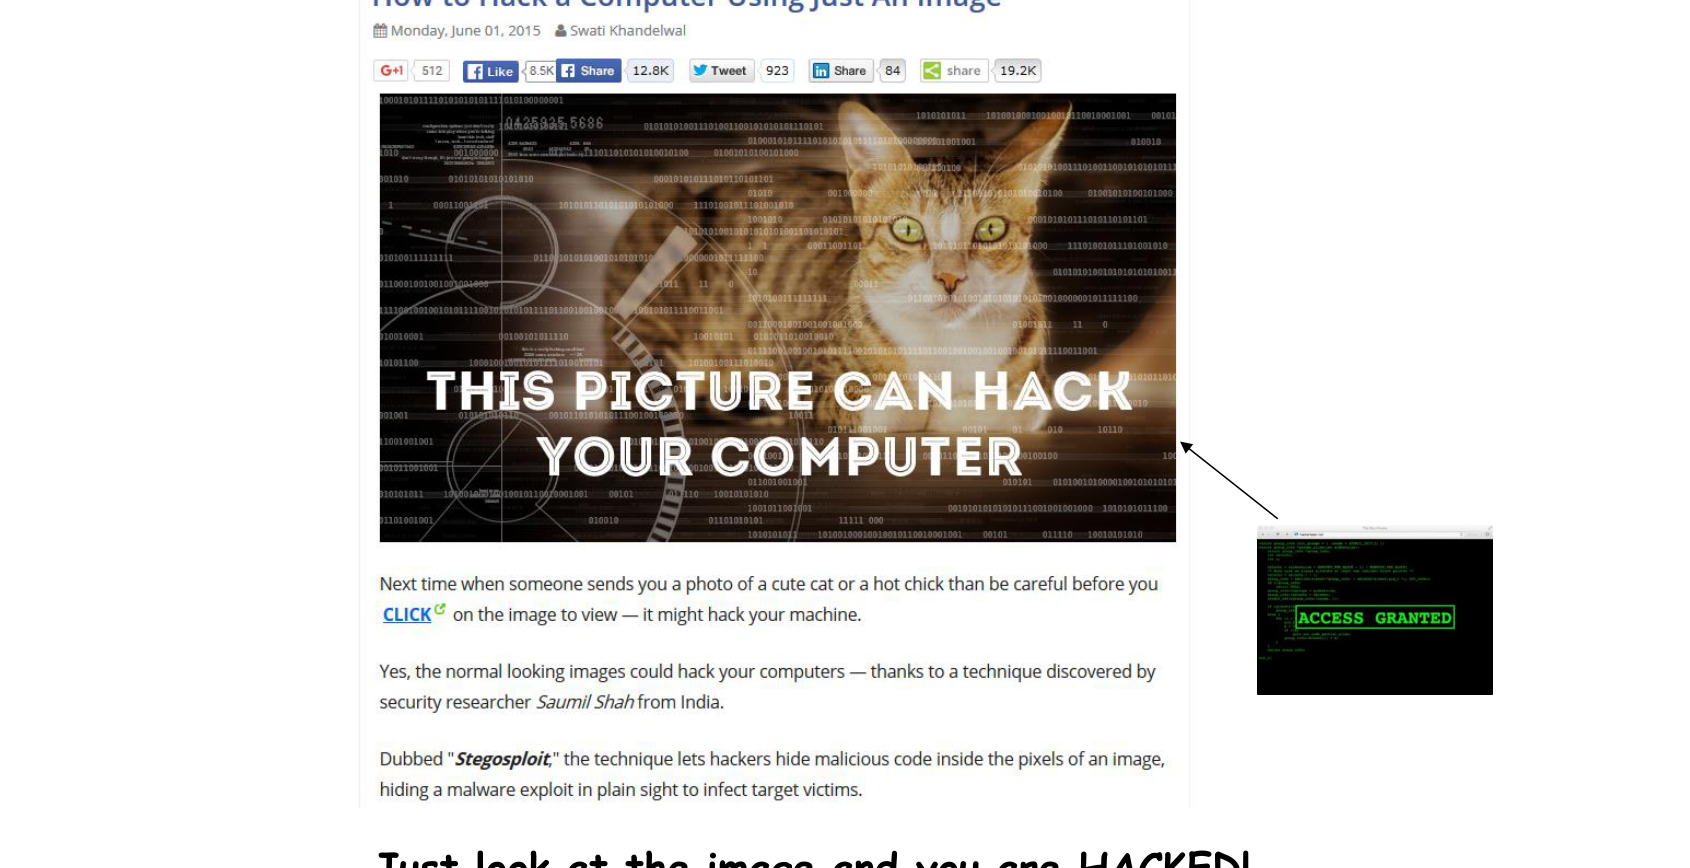
\includegraphics[width=184.80mm,height=238.79mm]{images/llm/page_008_img_01.png}%
\end{textblock*}

% deskripsi: Screenshot kecil yang menunjukkan terminal komputer dengan pesan 'ACCESS GRANTED' berwarna hijau.
% bbox normalisasi: [0.7220, 0.5880, 0.8420, 0.7250]
\begin{textblock*}{25.20mm}(151.62mm,174.64mm)
\noindent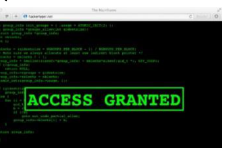
\includegraphics[width=25.20mm,height=40.69mm]{images/llm/page_008_img_02.png}%
\end{textblock*}

% bbox perkiraan otomatis: Screenshot artikel berita tentang Stegosploit yang menunjukkan gambar kucing dengan teks overlay 'THIS PICTURE CAN HACK YOUR COMPUTER' dan penjelasan mengenai teknik menyembunyikan kode berbahaya dalam piksel gambar.

\newpage

% --- unit llm 9 ---
% === Halaman 9 (llm) ===

\begin{itemize}
    \item Steganalisis diperlukan di dalam \textit{forensic image analysis}
    \item \textbf{Forensic Image Analysis} is the application of image science and domain expertise to interpret the \underline{content of} an image and/or the image itself in legal matters.
    \item Subdisiplin dari \textit{Forensic Image Analysis}:
    \begin{enumerate}
        \item Photogrammetry
        \item Photographic Comparison
        \item \underline{Content Analysis}
        \item \underline{Image Authentication}
    \end{enumerate}
\end{itemize}

\newpage

% --- unit llm 10 ---
% === Halaman 10 (llm) ===

\begin{itemize}
    \item Salah satu pekerjaan di dalam \textit{content analysis} adalah mendeteksi apakah ada pesan tersembunyi di dalam sebuah gambar.
    \item Contoh sebuah skenario: Mr. Abdul, seorang investigator forensik, diminta Lab Forensik Polri untuk menginvestigasi sebuah \textit{cybercrime} berupa foto. Sebagai investigator forensik yang ahli, dia menganalisis foto untuk menemukan pesan tersembunyi di dalamnya dengan kakas \underline{steganalisis}.
\end{itemize}
\vspace{10mm}

\vspace{74.84mm}

% deskripsi: Ilustrasi seorang investigator dengan balon teks yang menjelaskan fokus analisis: menemukan konten steganografi dan mengekstrak informasi dari file gambar.
% bbox normalisasi: [0.4820, 0.6160, 0.7480, 0.8680]
\begin{textblock*}{55.86mm}(101.22mm,182.95mm)
\noindent
\includegraphics[width=55.86mm,height=74.84mm]{images/llm/page_010_img_01.png}%
\end{textblock*}

\newpage

% --- unit llm 11 ---
% === Halaman 11 (llm) ===

\begin{itemize}
  \item Tujuan utama steganalisis adalah untuk membedakan apakah sebuah media mengandung pesan rahasia atau tidak.
  \item Steganalisis dianggap berhasil jika ia dapat menentukan apakah sebuah media mengandung pesan tersembunyi dengan peluang lebih tinggi daripada menerka secara acak.
  \item Selain tujuan utama di atas, terdapat beberapa tujuan minor steganalisis:
  \begin{itemize}
    \item menentukan panjang pesan
    \item menentukan tipe algoritma penyisipan
    \item kunci yang digunakan
  \end{itemize}
\end{itemize}

\newpage

% --- unit llm 12 ---
% === Halaman 12 (llm) ===

\section*{Jenis-jenis stegananalisis}

\textbf{1. Targeted stegananalysis}
\begin{itemize}
    \item Teknik stegananalisis yang bekerja pada algoritma steganografi spesifik, dan kadang-kadang dibatasi hanya pada format media tertentu saja.
    \item Teknik ini mempelajari dan menganalisis algoritma penyisipan, lalu menemukan statistik yang berubah setelah penyisipan.
    \item Hasil stegananalisis sangat akurat, tetapi tidak fleksibel karena tidak dapat diperluas untuk algoritma steganografi yang lain atau format media yang berbeda.
\end{itemize}

\newpage

% --- unit llm 13 ---
% === Halaman 13 (llm) ===

\section*{2. Blind stegananalysis}

\begin{itemize}
    \item Teknik steganalisis yang bekerja pada sembarang algoritma steganografi dan sembarang format media.
    \item Teknik ini mempelajari perbedaan antara statistik \textit{cover-object} dan \textit{stego-object} dan membedakannya. Proses pembelajaran (\textit{learning}) dilakukan dengan melatih (\textit{training}) mesin pada sekumpulan database media. Model \textit{machine learning} yang digunakan misalnya jaringan syaraf tiruan.
    \item Hasil steganalisis kurang akurat dibandingkan dengan teknik \textit{targeted steganalysis}, tetapi kelebihannya adalah dapat diperluas untuk algoritma yang lain.
\end{itemize}

\newpage

% --- unit llm 14 ---
% === Halaman 14 (llm) ===

\section*{Metode Steganalisis}

1. Serangan berbasis visual (\textit{visual attacks})
\begin{itemize}
    \item Khusus untuk \textit{stego-object} berupa citra
    \item Bersifat subjektif, karena melakukan pengamatan secara kasat mata dengan melihat artefak yang mencurigakan di dalam \textit{stego-image}, lalu membandingkannya dengan citra asli (\textit{cover image})
    \item Digunakan pada masa-masa awal riset steganalisis
    \item Contoh serangan visual:
    \begin{enumerate}
        \item \textit{LSB plane attack}
        \item \textit{Filtered visual attack} (Enhanced LSB)
    \end{enumerate}
\end{itemize}

\newpage

% --- unit llm 15 ---
% === Halaman 15 (llm) ===

\section*{2. Serangan berbasis statistik (statistical attack)}

\begin{itemize}
    \item Menggunakan analisis matematik pada citra untuk menemukan perbedaan antara \textit{cover image} dengan \textit{stego image}.
    \item Didasarkan pada fakta bahwa penyembunyian pesan ke dalam media menimbulkan artefak yang dapat dideteksi secara statistik sehingga dapat mengungkap penyembunyian pesan atau pesan yang disembunyikan itu sendiri.
    \item Contoh serangan statistik:
    \begin{enumerate}[a.]
        \item \textit{histogram analysis}
        \item \textit{Regular-singular (RS) analysis}
        \item \textit{Chi-square analysis}
        \item \textit{Sample pair (SP) analysis}
    \end{enumerate}
\end{itemize}

\newpage

% --- unit llm 16 ---
% === Halaman 16 (llm) ===

\section*{Visual Attack}

\begin{itemize}
    \item Memanfaatkan indera penglihatan $\rightarrow$ inspeksi kerusakan pada gambar akibat penyisipan
    \item Ide dasar :
\end{itemize}

\vspace{10mm}

% deskripsi: Diagram alir proses Visual Attack yang terdiri dari tiga kotak proses: 'media pembawa/ steganogram diserang' mengarah ke 'ekstraksi bit-bit yang berpotensi menjadi bit Pesan', yang kemudian mengarah ke 'Ilustrasi visual dari bit-bit yang telah diekstraksi dengan posisi yang sesuai dengan pixel sumbernya'.
% bbox normalisasi: [0.1980, 0.5510, 0.7610, 0.8760]
\begin{textblock*}{118.23mm}(41.58mm,163.65mm)
\noindent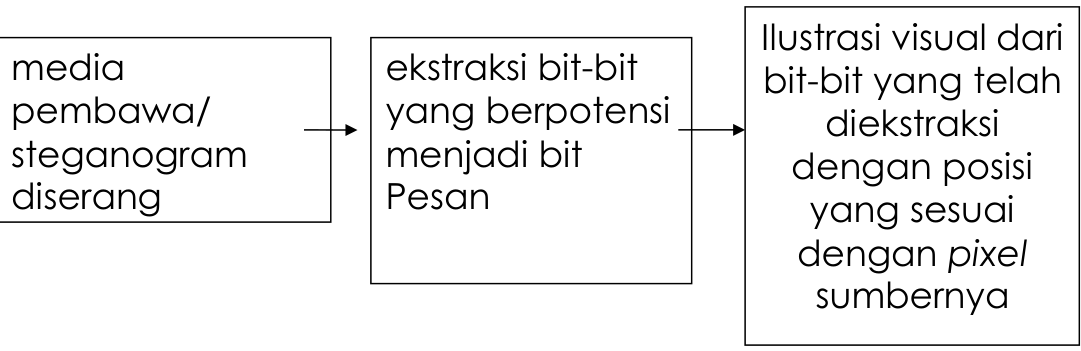
\includegraphics[width=118.23mm,height=96.52mm]{images/llm/page_016_img_01.png}%
\end{textblock*}

\newpage

% --- unit llm 17 ---
% === Halaman 17 (llm) ===

\vspace{129.79mm}

Metode Enhanced LSB

% deskripsi: Ilustrasi proses modifikasi bit LSB (Least Significant Bit) pada komponen warna Blue, Green, dan Red, menunjukkan perubahan nilai biner dari warna asli menjadi nilai maksimal atau minimal.
% bbox normalisasi: [0.1580, 0.2740, 0.8370, 0.3980]
\begin{textblock*}{142.59mm}(33.18mm,81.38mm)
\noindent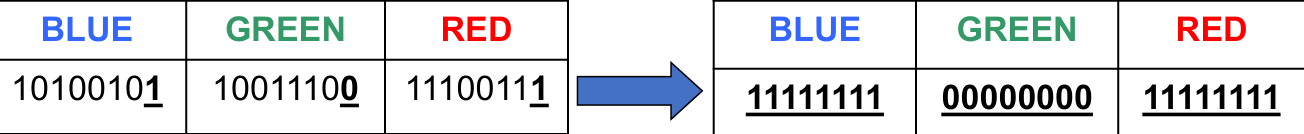
\includegraphics[width=142.59mm,height=36.83mm]{images/llm/page_017_img_01.png}%
\end{textblock*}

% deskripsi: Perbandingan gambar kincir angin sebelum (kiri) dan sesudah (kanan) diterapkan metode Enhanced LSB, di mana gambar kanan menunjukkan noise warna yang signifikan.
% bbox normalisasi: [0.1930, 0.4750, 0.7780, 0.9120]
\begin{textblock*}{122.85mm}(40.53mm,141.07mm)
\noindent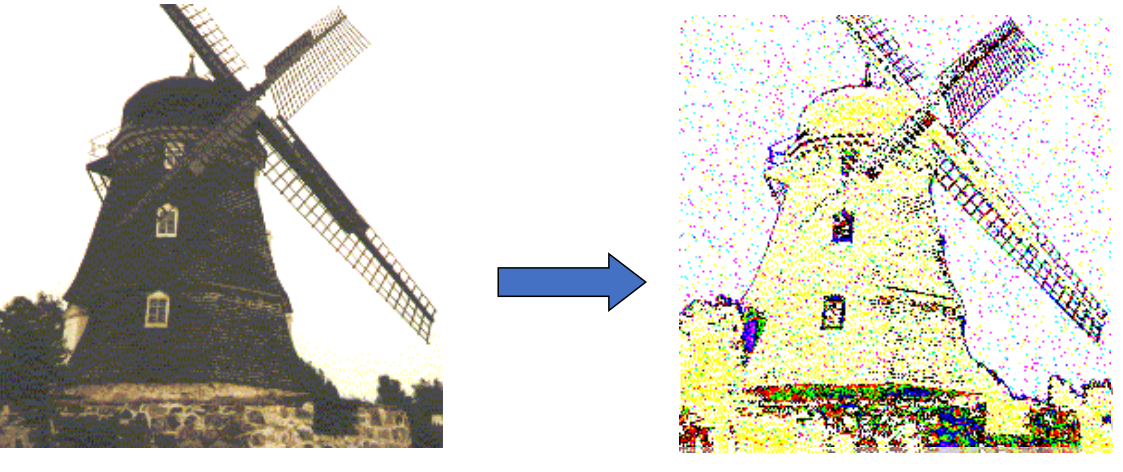
\includegraphics[width=122.85mm,height=129.79mm]{images/llm/page_017_img_02.png}%
\end{textblock*}

\newpage

% --- unit llm 18 ---
% === Halaman 18 (llm) ===

\vspace{127.71mm}

(a) Citra orisinal \vspace{10mm} (b) Citra hasil enhanced LSB \vspace{10mm} (c) Citra stego \vspace{10mm} (b) Citra hasil enhanced LSB

\vspace{100.98mm}

% deskripsi: Ilustrasi proses steganografi: Gambar (a) menampilkan citra orisinal Doraemon, panah biru mengarah ke gambar (b) yang menunjukkan hasil ekstraksi bit LSB (enhanced LSB) yang terlihat seperti noise berwarna.
% bbox normalisasi: [0.2480, 0.0900, 0.7050, 0.5200]
\begin{textblock*}{95.97mm}(52.08mm,26.73mm)
\noindent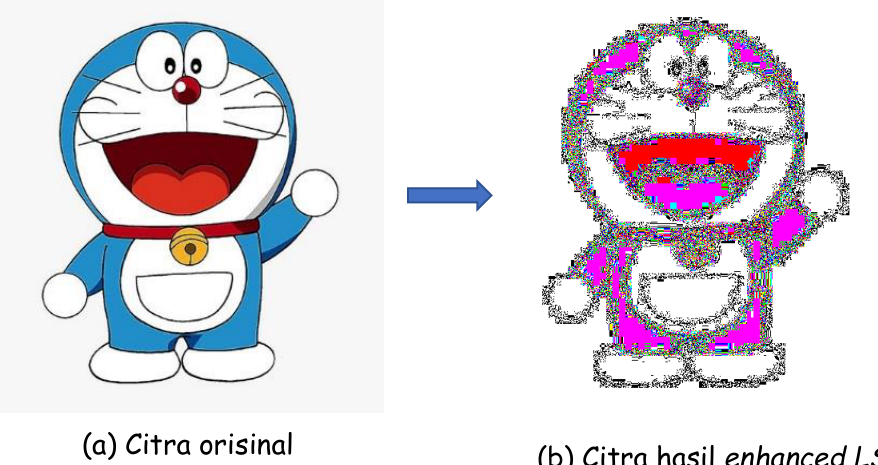
\includegraphics[width=95.97mm,height=127.71mm]{images/llm/page_018_img_01.png}%
\end{textblock*}

% deskripsi: Ilustrasi proses steganografi: Gambar (c) menampilkan citra stego (citra yang sudah disisipi pesan), panah biru mengarah ke gambar (b) di bawahnya yang menunjukkan hasil ekstraksi bit LSB (enhanced LSB).
% bbox normalisasi: [0.2780, 0.5500, 0.7220, 0.8900]
\begin{textblock*}{93.24mm}(58.38mm,163.35mm)
\noindent
\includegraphics[width=93.24mm,height=100.98mm]{images/llm/page_018_img_02.png}%
\end{textblock*}

\newpage

% --- unit llm 19 ---
% === Halaman 19 (llm) ===

\begin{center}
\textbf{Teknik Steganalisis: Visual Attack}
\end{center}

\vspace{10mm}

\begin{center}
\begin{tabular}{cccc}
Gambar asli & Hasil penapisan (asli) & Terdeteksi ada pesan & Terdeteksi ada pesan
\end{tabular}
\end{center}

\vspace{10mm}

\begin{center}
\begin{tabular}{cc}
Terdeteksi ada pesan & Terdeteksi ada pesan
\end{tabular}
\end{center}

% deskripsi: Kumpulan gambar contoh visual attack pada steganografi, menampilkan gambar asli kincir angin, hasil penapisan, dan beberapa variasi deteksi pesan dengan artefak visual berupa noise warna-warni.
% bbox normalisasi: [0.1600, 0.2300, 0.8800, 0.5500]
\begin{textblock*}{151.20mm}(33.60mm,68.31mm)
\noindent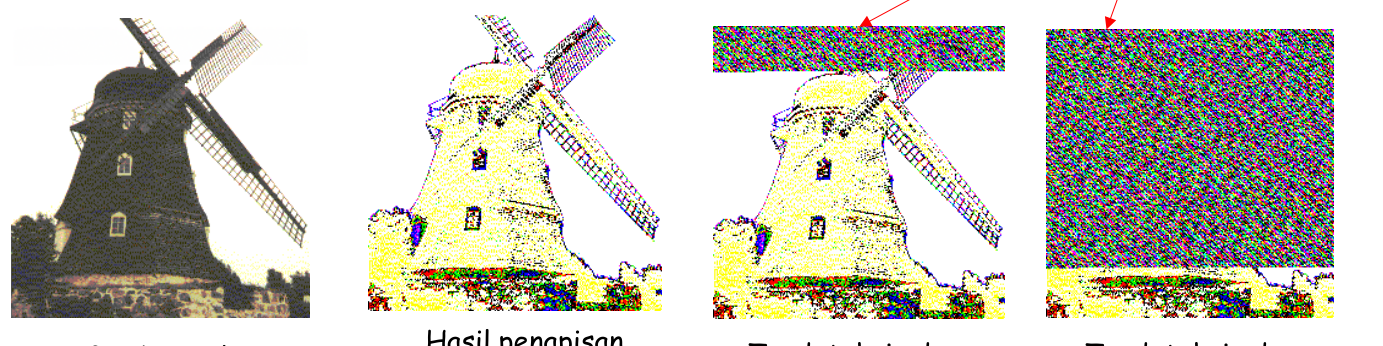
\includegraphics[width=151.20mm,height=95.04mm]{images/llm/page_019_img_01.png}%
\end{textblock*}

% deskripsi: Dua contoh gambar tambahan yang menunjukkan deteksi adanya pesan melalui analisis visual dengan noise warna-warni.
% bbox normalisasi: [0.2400, 0.6300, 0.6900, 0.9100]
\begin{textblock*}{94.50mm}(50.40mm,187.11mm)
\noindent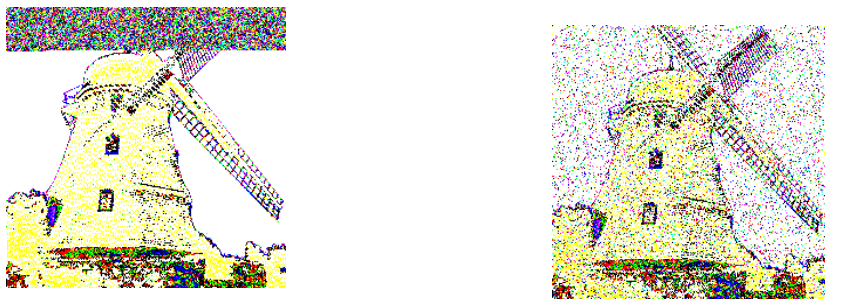
\includegraphics[width=94.50mm,height=83.16mm]{images/llm/page_019_img_02.png}%
\end{textblock*}

\newpage

% --- unit llm 20 ---
% === Halaman 20 (llm) ===

Metode enhanced-LSB bagus untuk citra dengan kontras tinggi, yaitu citra yang memiliki warna latar yang jelas atau memiliki perbedaan warna yang kontras antara latar dengan gambar utama

\vspace{20mm}

Gambar III-1 Gambar yang mengandung pesan rahasia dan hasil enhanced LSB-nya [PAU07]

% deskripsi: Perbandingan antara citra asli yang mengandung pesan rahasia dan hasil ekstraksi menggunakan metode enhanced LSB.
% bbox normalisasi: [0.2200, 0.5300, 0.7700, 0.7600]
\begin{textblock*}{115.50mm}(46.20mm,157.41mm)
\noindent
\includegraphics[width=115.50mm,height=68.31mm]{images/llm/page_020_img_01.png}%
\end{textblock*}

\newpage

% --- unit llm 21 ---
% === Halaman 21 (llm) ===

Untuk citra dengan kontras rendah (seperti citra hasil fotografi), metode \textit{enhanced LSB} seringkali menyulitkan steganalisis. Karena steganalisis akan kesulitan membedakan antara gambar yang seharusnya muncul dengan pesan rahasia.\vspace{10mm}

\vspace{117.32mm}

Gambar III-3 Gambar dengan kontras rendah dan hasil \textit{enhanced LSB}-nya

% deskripsi: Perbandingan antara citra asli berupa bunga teratai (kontras rendah) di sisi kiri dan hasil pengolahan enhanced LSB yang terlihat seperti noise berwarna di sisi kanan.
% bbox normalisasi: [0.2020, 0.3720, 0.7520, 0.7670]
\begin{textblock*}{115.50mm}(42.42mm,110.48mm)
\noindent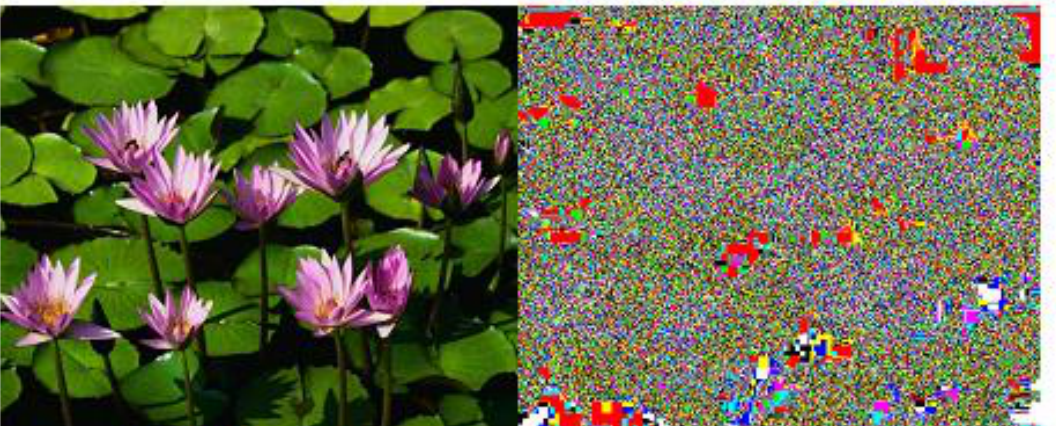
\includegraphics[width=115.50mm,height=117.32mm]{images/llm/page_021_img_01.png}%
\end{textblock*}

\newpage

% --- unit llm 22 ---
% === Halaman 22 (llm) ===

\section*{NoStega: Noiseless Steganography}

\begin{itemize}
    \item Teknik baru steganografi, ditemukan oleh Desoky (2012)
    \item Tidak membutuhkan \textit{cover} untuk menyembunyikan pesan
    \item Latar belakang: penyembunyian pesan di dalam \textit{cover} dapat membuat kualitas \textit{cover} menjadi terdegradasi $\implies$ dapat diserang secara steganalisis untuk menemukan \textit{embedded message}

    \item \textit{NoStega} melakukan kamuflase dengan cara menyembunyikan pesan dalam bentuk \textit{cover} yang terlihat alami sehingga tidak menimbulkan kecurigaan.

    \item \textit{NoStega} menggunakan berbagai materi untuk melakukan kamuflase seperti grafik, email, game, catatan, dan lain-lain.
\end{itemize}

\newpage

% --- unit llm 23 ---
% === Halaman 23 (llm) ===

\section*{GraphStega (Graph Steganography)}

\begin{itemize}
    \item Salah satu teknik di dalam \textit{NoStega}
    \item Melakukan kamuflase dengan cara mengubah pesan menjadi plot pada grafik.
    \item Contoh: pesan rahasia \textcolor{red}{"Use my secret key"}.
    Ubah pesan ke dalam biner:
\end{itemize}

\begin{center}
    \textcolor{red}{\texttt{010101010111001101100101010010000000110110101011110010}}\
    \textcolor{red}{\texttt{010000000111001101100101010110001101111001001100101011}}\
    \textcolor{red}{\texttt{101000010000000110101011011001010101111001}}
\end{center}

\newpage

% --- unit llm 24 ---
% === Halaman 24 (llm) ===

\begin{itemize}
    \item Selanjutnya, kelompokkan menjadi kelompok-kelompok 7 bit:
    
    \vspace{5mm}
    \textcolor{red}{0101010 1011100 1101100 1010010 0000011 0110101 1110010}
    \textcolor{red}{0100000 0111001 1011001 0101100 0110111 0010011 0010101}
    \textcolor{red}{1101000 0100000 0110101 1011001 0101111 001}
    
    \vspace{10mm}
    \item Konversi kelompok-kelompok 7-bit di atas menjadi nilai desimal
    
    \vspace{5mm}
    \textcolor{red}{42 92 108 82 3 53 114 32 57 89 44 55 19 21 104 32 53 89 47 1.}
\end{itemize}

\newpage

% --- unit llm 25 ---
% === Halaman 25 (llm) ===

\begin{itemize}
  \item Buatlah grafik dengan Microsoft Excell dengan menggunakan nilai-nilai desimal di atas
  \item Misalnya nilai-nilai tersebut menyatakan jumlah penderita demam berdarah selama 20 bulan di Kota Bogor (Januari 2017 -- Agustus 2018).
\end{itemize}

\vspace{10mm}

% deskripsi: Grafik batang yang menunjukkan jumlah penderita Demam Berdarah di Kota Bogor dari Januari 2017 sampai Agustus 2018.
% bbox normalisasi: [0.2010, 0.3450, 0.7860, 0.9840]
\begin{textblock*}{122.85mm}(42.21mm,102.46mm)
\noindent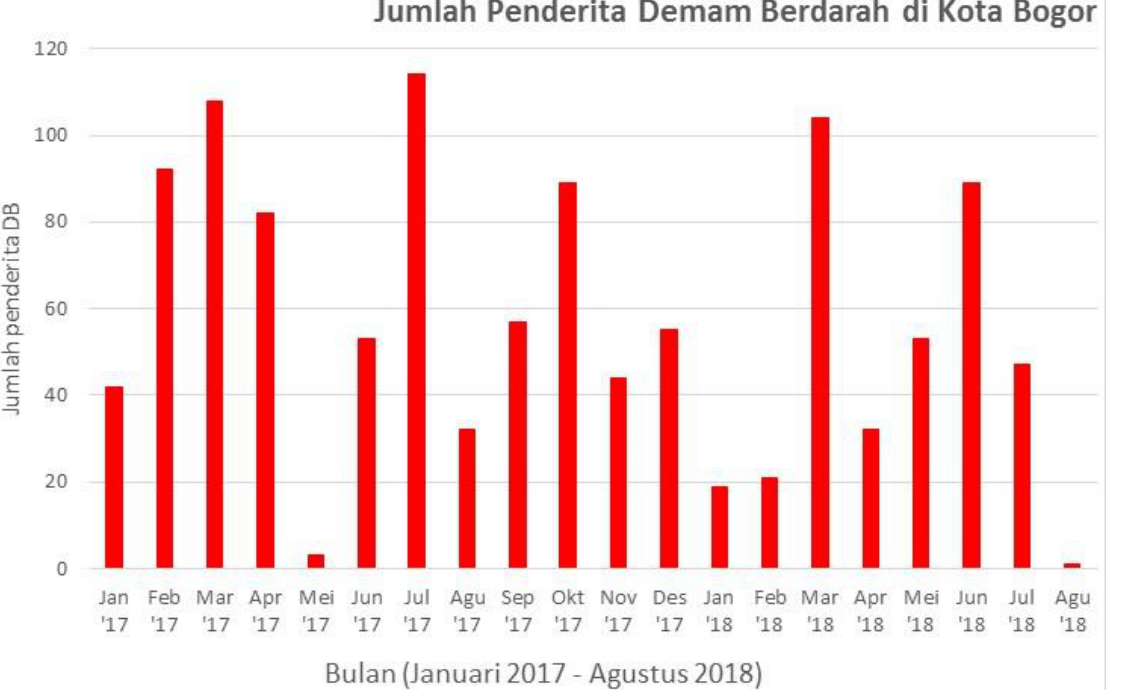
\includegraphics[width=122.85mm,height=189.78mm]{images/llm/page_025_img_01.png}%
\end{textblock*}

\newpage

% --- unit llm 26 ---
% === Halaman 26 (llm) ===

\vspace{213.84mm}

Alternatif grafik lainnya:

% deskripsi: Grafik garis yang menunjukkan Jumlah Penderita Demam Berdarah di Kota Bogor dari Januari 2017 hingga Agustus 2018, dengan fluktuasi jumlah kasus per bulan.
% bbox normalisasi: [0.1700, 0.2000, 0.8200, 0.9200]
\begin{textblock*}{136.50mm}(35.70mm,59.40mm)
\noindent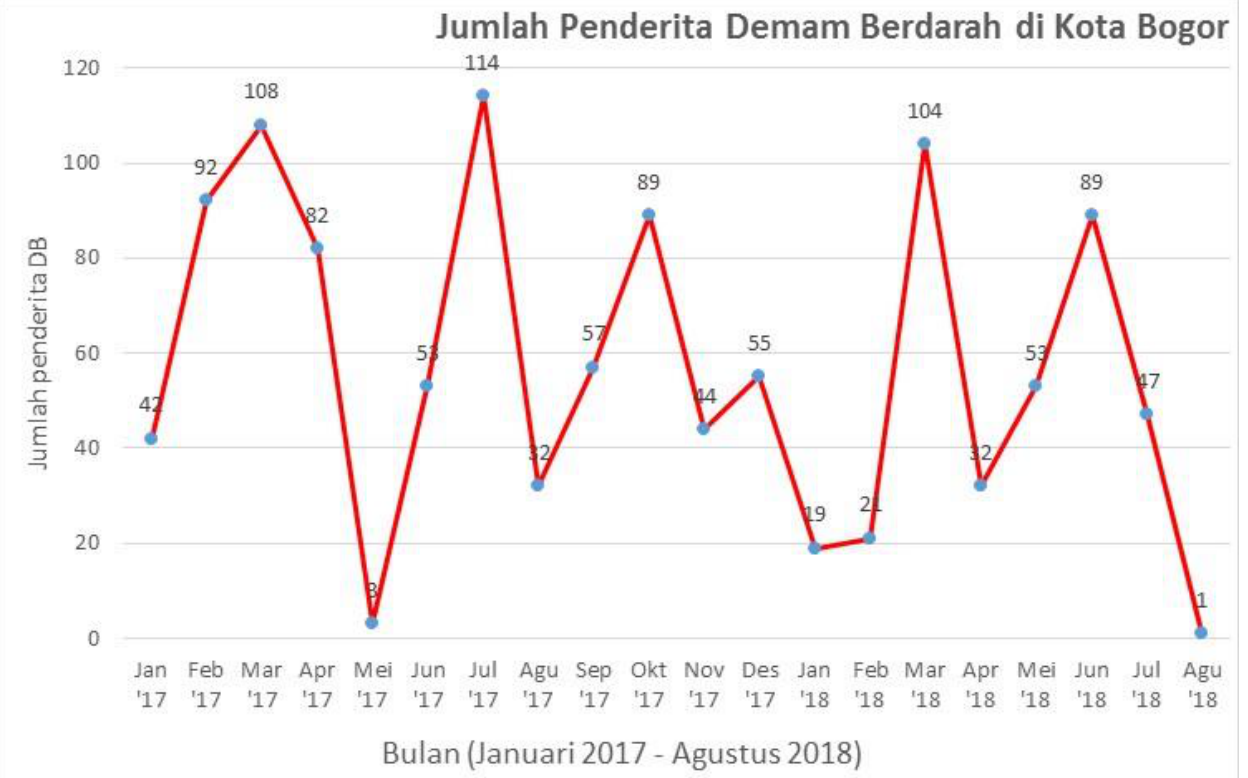
\includegraphics[width=136.50mm,height=213.84mm]{images/llm/page_026_img_01.png}%
\end{textblock*}

\newpage

% --- unit llm 27 ---
% === Halaman 27 (llm) ===

Untuk membaca pesan rahasia, penerima membaca nilai-nilai pada grafik,

42 92 108 82 3 53 114 32 57 89 44 55 19 21 104 32 53 89 47 1

lalu mengubahnya ke dalam biner,

00101010 01011100 01101100 01010010 00000011 00110101 01110010\\
00100000 00111001 01011001 00101100 00110111 00010011 00010101\\
01101000 00100000 00110101 01011001 0101111 0001

Untuk setiap kelompok biner ambil 7-bit dari belakang (7-bit LSB),

0101010 1011100 1101100 1010010 0000011 0110101 1110010\\
0100000 0111001 1011001 0101100 0110111 0010011 010101\\
1101000 0100000 0110101 1011001 0101111 001

\newpage

% --- unit llm 28 ---
% === Halaman 28 (llm) ===

Gabungkan semua kelompok bit menjadi satu,\\
\textcolor{red}{0101010101110011011001001010010000000110110101011110010}\\
\textcolor{red}{010000000111001101100100101011000110111100100100100101011}\\
\textcolor{red}{1010000100000000110101011011001010101111001}\\
\vspace{10mm}
Kemudian kelompokkan menjadi kelompok-kelompok 8-bit,\\
\textcolor{red}{01010101 01110011 01100101 00100000 01101101 01111001}\\
\textcolor{red}{00100000 01110011 01100101 01100011 01110010 01100101}\\
\textcolor{red}{01110100 00100000 01101011 01100101 01111001}\\
\vspace{10mm}
Kodekan setiap delapan bit tersebut menjadi karakter ASCII\\
\textcolor{red}{Use my secret key}\\
\vspace{10mm}
Pesan rahasia berhasil dibaca kembali!

\newpage

% --- unit llm 29 ---
% === Halaman 29 (llm) ===

\section*{Teknik NoStega lainnya}

\vspace{94.45mm}

\begin{enumerate}
  \item[3.] Nc3 \quad Nf6
  \item[4.] exd5 \quad exd5
  \item[5.] Nf3 \quad Bd6
  \item[6.] Bd3 \quad O-O
  \item[7.] O-O \quad h6
  \item[8.] Re1 \quad Nc6
  \item[9.] Nb5 \quad Bb4
  \item[10.] c3 \quad Ba5
  \item[11.] Na3 \quad Bg4
  \item[12.] Nc2 \quad Qd7
  \item[13.] b4 \quad Bb6
  \item[14.] h3 \quad Bb5
  \item[15.] Ne3 \quad Rfe8
  \item[16.] b5 \quad Nc7
  \item[17.] g4 \quad Bg6
  \item[18.] Ne5 \quad Qc8
  \item[19.] a4 \quad c6
  \item[20.] bxc6 \quad bxc6
  \item[21.] Ba3 \quad Ne4
  \item[22.] Qc2 \quad Ng5
  \item[23.] Bxe7 \quad Rxe7
  \item[24.] Bxg6 \quad Bxg6
  \item[25.] Qxg6 \quad Nxh3+
  \item[26.] Kh2 \quad Nf4
  \item[27.] Qf5 \quad Ne6
  \item[28.] Ng2 \quad Qc7
\end{enumerate}

\vspace{10mm}

\begin{center}
\textcolor{red}{Chess-stega} \quad \quad \quad \quad \quad \quad \quad \textcolor{red}{Head-stega}
\end{center}

% deskripsi: Screenshot papan catur sebagai ilustrasi teknik Chess-stega
% bbox normalisasi: [0.1780, 0.3220, 0.3540, 0.6400]
\begin{textblock*}{36.96mm}(37.38mm,95.63mm)
\noindent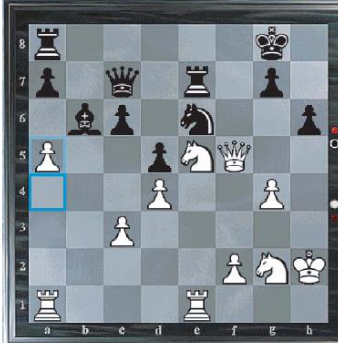
\includegraphics[width=36.96mm,height=94.45mm]{images/llm/page_029_img_01.png}%
\end{textblock*}

% deskripsi: Screenshot jendela email sebagai ilustrasi teknik Head-stega
% bbox normalisasi: [0.4620, 0.3140, 0.9450, 0.6520]
\begin{textblock*}{101.43mm}(97.02mm,93.26mm)
\noindent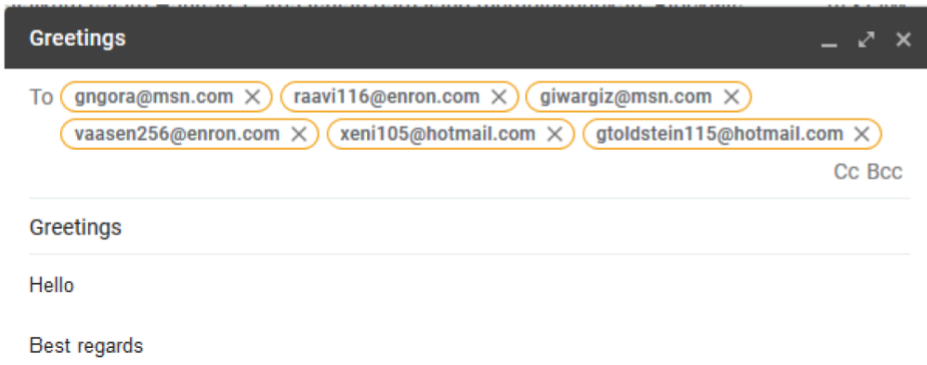
\includegraphics[width=101.43mm,height=100.39mm]{images/llm/page_029_img_02.png}%
\end{textblock*}

\newpage

% --- unit llm 30 ---
% === Halaman 30 (llm) ===

\vspace{177.61mm}

Ada pertanyaan?

% deskripsi: Foto hitam putih sekelompok siswa di dalam kelas yang mengangkat tangan mereka untuk bertanya atau menjawab.
% bbox normalisasi: [0.1850, 0.2500, 0.7740, 0.8480]
\begin{textblock*}{123.69mm}(38.85mm,74.25mm)
\noindent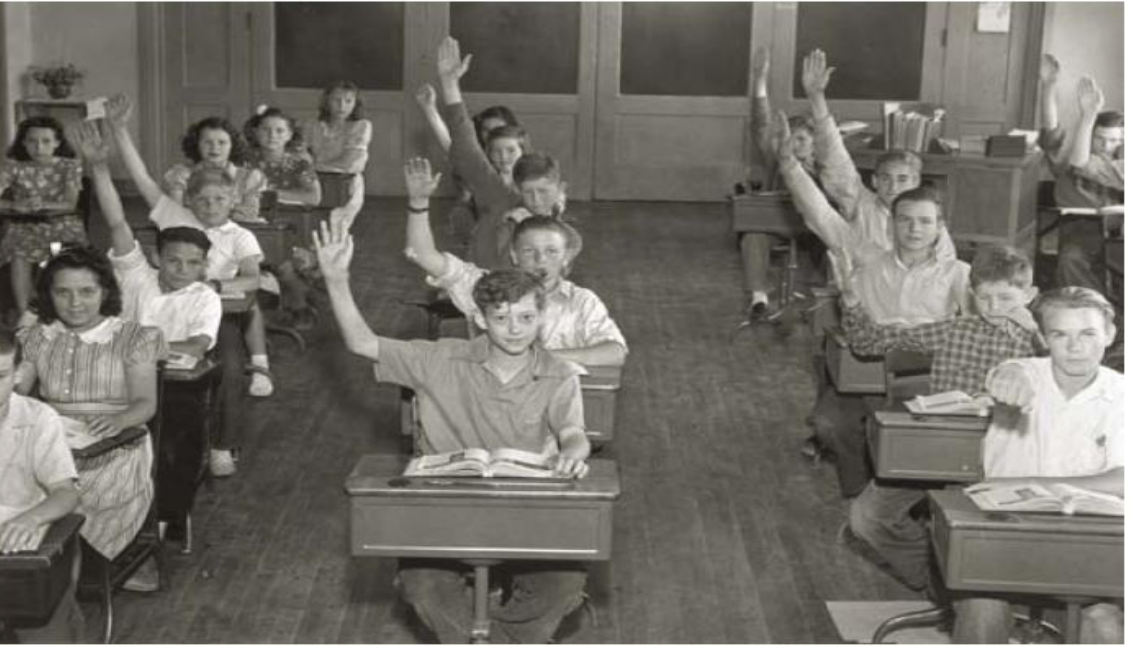
\includegraphics[width=123.69mm,height=177.61mm]{images/llm/page_030_img_01.png}%
\end{textblock*}

\end{document}
